\begin{figure}[hp]
    \centering
    \begin{subfigure}[h]{\floatwidth}
        \showthe\textwidth
          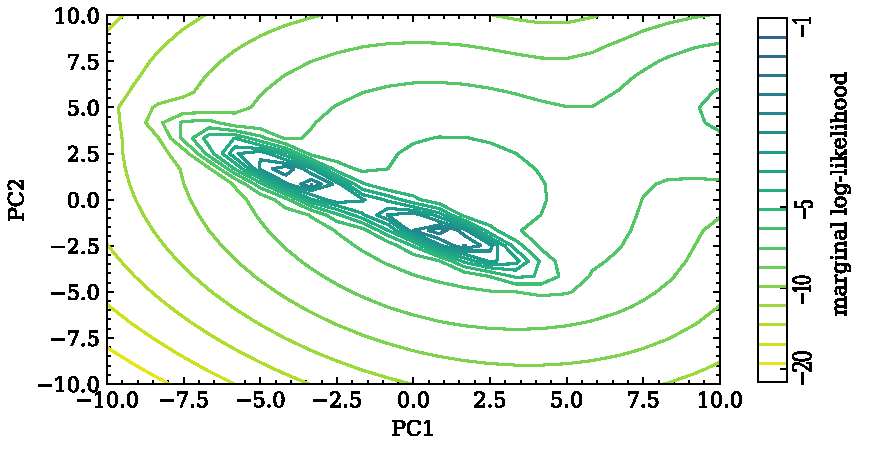
\includegraphics[width=\textwidth]{c3Bsle/Figs/densityestimation/de_pc1_pc2.pdf}
          \caption{First and second principal components}
    \end{subfigure}
  	\begin{subfigure}[h]{\floatwidth}
  	    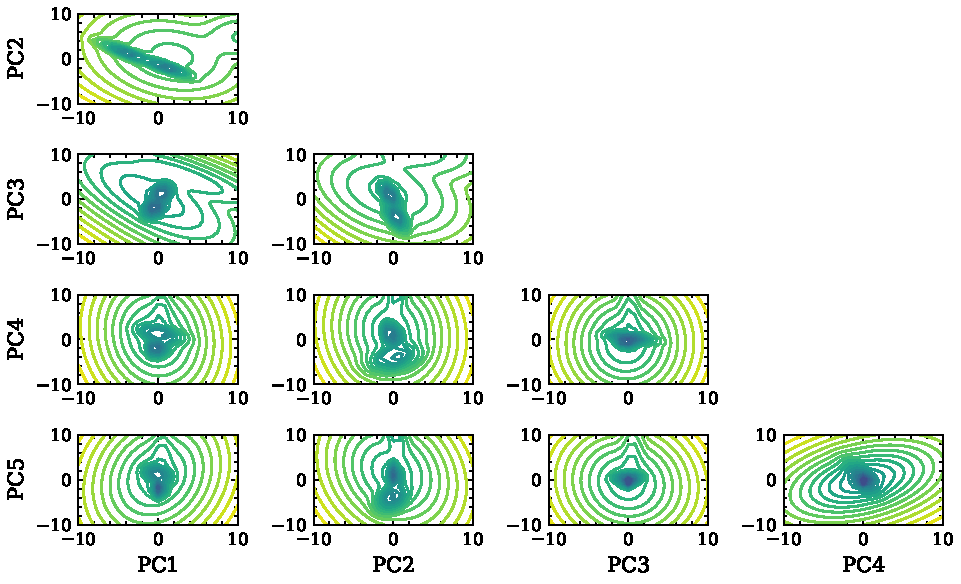
\includegraphics[width=\textwidth]{c3Bsle/Figs/densityestimation/de_pc_pair_plot.pdf}
  	    \caption{Pair plots for the first five principal components}
  	\end{subfigure}
    \Caption{Contour plots for multidimensional density estimation}{An estimator $\hat{p}(e_t)$ is computed using a GMM with 4 components fit to the first 5 principal components of the data as represented by GP hyperparameters. The contour plot of $\log \hat{p}(e_t)$ is shown for every pair of principal components by marginalizing 
    over the remaining axes. The regions with lower likelihood are more likely to be classified as seizures.}
    \label{fig:3bsle:de}
\end{figure}

